\documentclass{article}

\usepackage[utf8]{inputenc}
\usepackage{tikz}
\usepackage{amsmath}
\usepackage{mathtools}
\usepackage{amsfonts}
\usepackage{amssymb}
\usepackage{sectsty}
\usepackage{xcolor}
\usepackage[paperwidth=180mm, paperheight=290mm, left=10mm, top=10mm, bottom=10mm, right=10mm, margin=10mm]{geometry}
\usepackage{ragged2e}
\usepackage{listings}
\usepackage[hidelinks]{hyperref}

\definecolor{def}{RGB}{255, 150, 89}
\definecolor{tit}{RGB}{217, 84, 80}
\definecolor{emp}{RGB}{150, 206, 180}
\definecolor{acc}{RGB}{255, 234, 150}
\definecolor{txt}{RGB}{249, 232, 232}
\definecolor{back}{RGB}{22, 22, 22}

\sectionfont{\fontsize{20.74}{35}\ttfamily}
\subsectionfont{\color{tit}\fontsize{17.28}{17.28}\ttfamily}

\DeclareFontFamily{\encodingdefault}{\ttdefault}{
  \hyphenchar\font=\defaulthyphenchar
  \fontdimen2\font=0.33333em
  \fontdimen3\font=0.16667em
  \fontdimen4\font=0.11111em
  \fontdimen7\font=0.11111em
}

\newcommand{\R}{\mathbb{R}}
\newcommand{\N}{\mathbb{N}}
\newcommand{\Q}{\mathbb{Q}}
\newcommand{\Z}{\mathbb{Z}}
\newcommand{\C}{\mathbb{C}}
\newcommand{\cont}{\mathfrak{c}}

\geometry{a4paper, textwidth=155mm, textheight=267mm, left=15mm, top=15mm, right=15mm, marginparwidth=0mm}
\setlength\parindent{15pt}

\pagestyle{empty}

\begin{document}\pagecolor{back}\color{txt}\ttfamily
\section*{\color{tit}WSTEP DO WPROWADZENIA DO TEORII ZBIOROW}
\begin{center}\color{emp}\emph{Ze wstepem do matematyki jest jak z uswiadamianiem seksualnym dzieci - mowi \\im sie prawde, ale nie mowi im sie wszystkiego}\end{center}
\subsection*{\color{tit}ORGANIZACJA}
  \color{def}ZASADY ZALICZENIA\color{txt}\par
  - \color{acc}EGZAMIN USTNY\color{txt}\par
  - dwa kolokwia na poczatku maja i pod koniec semestru, zalezy kiedy uda sie zrobic listy\medskip\\
  \color{def}CZESCI WYKLADU\color{txt}\par
  - aksjomaty\par
  - liczby porzadkowe\par
  - aksjomat wyboru\par
  - liczby kardnalne\par
  - arytmetyka kardynalna\medskip\\
  \color{def}LITERATURA\color{txt}\par
  - J.Kraszewski \emph{Wstep do matematyki} (pierwsze wydanie ma duzo bledow)\par
  - A. Blaszczyk i M. Turek \emph{Teoria mnogosci}\par
  - Just, Weese \emph{Discovering Modern Set Theory} part I\bigskip\\
  jedyna poprawna strona internetowa: \href{https://math.uni.wroc.pl/~kraszew/}{\color{emp}math.uni.wroc.pl/~kraszew}
\subsection*{\color{tit}FUNKCJE}
  \begin{center}\color{def}FUNKCJA \color{txt}- zbior par uporzadkowanych o wlasnosci \emph{jednoznacznosci}, \\czyli nie ma dwoch par o tym samym poprzedniku i dwoch roznych nastepnikach\end{center}
  dziedzine i przeciwdziedzine okreslamy poza definicja funkcji - nie sa na tym samym poziomie co sama funkcja:
  $$\begin{matrix}\texttt{dom}(f)=\{x: \exists\;y\;\langle x, y\rangle \in f\}\\\texttt{rng}(f)=\{y: \exists\;x\;\langle x, y\rangle\in f\}\end{matrix}$$\\
  warto pamietac, ze \color{acc}definicja funkcji \color{txt}jako \emph{podzbioru $f\subseteq X\times Y$ taki, ze dla kazdego $x\in X$ istnieje dokladnie jeden $y\in Y$ takie, ze $\langle x, y\rangle \in f$} jest tak samo poprawna definicja, tylko \color{emp}kladzie nacisk na inny aspekt \color{txt}funkcji
\subsection*{\color{tit}OPERACJE UOGOLNIONE}
  dla \color{def}rodziny indeksowanej \color{txt}$\{A_i:i\in I\}$ definiujemy:\smallskip\par
  - jej sume: $\bigcup\limits_{i\in I}A_i=\{x:\;\exists\;i\in I \quad x\in A_i\}$\smallskip\par
  - jej przekroj: $\bigcap\limits_{i\in I}A_i=\{x:\;\forall\; i\in I\quad x\in A_i\}$\medskip\\
  sume uogolniona i przekroj uogolniony mozna definiowac na nieindeksowanej \color{acc}rodzinie zbiorow $\mathcal{A}$\color{txt}:\smallskip\par
  - suma: $\bigcup\mathcal{A}=\{x:\;\exists\;A\in\mathcal{A}\quad x\in A\}$\smallskip\par
  - przekroj: $\bigcap\mathcal{A}=\{x:\;\forall\; A\in\mathcal{A}\quad x\in A\}$\medskip\\
  \color{def}UOGOLNIONY ILOCZYN KARTEZJANSKI \color{txt}(uogolniony proodukt) zbiorow\\
  $$A_1\times A_2 =\{\langle x,y\rangle : x\in A_1 \land y\in A_2\}$$
  $$A_1\times A_2\times A_3 =\{\langle x,y, z\rangle : x\in A_1 \land y\in A_2\land z\in A_3\}$$
  pierwszym pomyslem na definiowanie iloczynu kartezjanskiego trzech zbiorow jest:
  $$A_1\times A_2\times A_3 :=(A_1\times A_2)\times A_3$$
  \color{emp}problem \color{txt}- czy iloczyn kartezjanski jest laczny?\\
  intuicyjnie tak, formalnie juz nie:
  $$(A_1\times A_2)\times A_3\neq A_1\times (A_2\times A_3)$$
  bo byty sa inne:
  $$\langle\langle a_1, a_2\rangle, a_3\rangle \neq \langle a_1, \langle a_2, a_3\rangle\rangle$$\medskip
  \begin{center}\emph{\color{emp}mimo ze iloczyn kartezjanski nie jest laczny, matematycy nie maja \\problemu uznawac, ze jest laczny}\smallskip\\
  \color{def}ISTNIEJE NATURALNA, KANONICZNA, BIJEKCJA\color{txt}, \\ktora lewej stronie intuicyjnie przypisuje prawa strone\end{center}
  Formalnie \color{acc}indeksowana rodzina zbiorow \color{txt}jest funkcja ze zbioru indeksow w rodzine zbiorow, wiec powinna byc zapisywana w \color{acc}nawiasach trojkatnych. \color{txt}\\
  Zapis w \color{acc}klamrach oznacza zbior wartosci \color{txt}tej funkcji i nie ma znaczenia czy dany zbior pojawia sie jeden czy 30 razy - nie przeszkadza to definiowac sumy czy przekroju\medskip\\
  $\langle A_i:i\in I\rangle$ - indeksowana rodzina zbiorow, czyli \color{acc}$A: I\to \bigcup\limits_{i\in I}\;A_i\quad A(i)=A_i$\color{txt}\medskip\\
  Wyobrazmy sobie iloczyn kartezjanskich dwoch zbiorow nie jako punkt na plaszczyznie, a jako dwuelementowy ciag:
  \begin{center}\begin{tikzpicture}
    \node(p) at (0, 0) {$A_1$};
    \node(k) at (2, 0) {$A_2$};
    \draw[white, thick] (p)--(0, 2);
    \draw[white, thick] (k)--(2, 2);
    \node(a11) at(0, 1) {$\circ$};
    \node(a22) at(2, 1.5) {$\circ$};
    \node(a1) at (-0.3, 1) {$a_1$};
    \node(a2) at (2.3, 1.5) {$a_2$};
    \draw[yellow, thick] (a11)--(a22);
  \end{tikzpicture}\end{center}
  To przedstawienie latwo przelozyc na nieskonczenie dlugi iloczyn kartezjanski - dorysowuje sie kolejna os z elementami kolejnego podozbioru rodziny:
  \begin{center}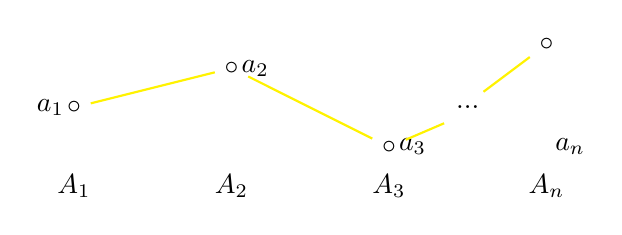
\begin{tikzpicture}
    \node(p) at (0, 0) {$A_1$};
    \node(k) at (2, 0) {$A_2$};
    \node(b) at (4, 0) {$A_3$};
    \node(m) at (6, 0) {$A_n$};
    \draw[white, thick] (p)--(0, 2);
    \draw[white, thick] (k)--(2, 2);
    \draw[white, thick] (b)--(4, 2);
    \draw[white, thick] (m)--(6, 2);
    \node(a11) at(0, 1) {$\circ$};
    \node(a22) at(2, 1.5) {$\circ$};
    \node(a33) at(4, 0.5) {$\circ$};
    \node(ann) at(6, 1.8) {$\circ$};
    \node(a1) at (-0.3, 1) {$a_1$};
    \node(a2) at (2.3, 1.5) {$a_2$};
    \node(a3) at (4.3, 0.5) {$a_3$};
    \node(kropecki) at (5, 1) {...};
    \node(an) at (6.3, 0.5) {$a_n$};
    \draw[yellow, thick] (a11)--(a22);
    \draw[yellow, thick] (a22)--(a33);
    \draw[yellow, thick] (a33)--(4.7, 0.8);
    \draw[yellow, thick] (ann)--(5.2, 1.2);
  \end{tikzpicture}\end{center}
  W ten sposob powstaje funkcja, ktora kolejnym inteksom przypisuje element z tego indeksu:
  $$f:I\to\bigcup\limits_{i\in I}A_i$$
  $$f(i) \in A_i$$
  \begin{center}
    wiec \color{def}iloczyn uogolniony to zbior funkcji \color{txt}ze zbioru \\indeksowego w rodzine indeksowana\smallskip\\
    $\prod\limits_{i\in I}A_i=\{f\in(\bigcup\limits_{i\in I}A_i)^I:\;\forall\;f(i)\in A_i\}$
  \end{center}
  AAAALEEEE
  $$\prod\limits_{i\in I}A_i\neq A_1\times A_2\quad I=\{1, 2\}$$
  Po lewej mamy zbior funkcji, a po prawej mamy iloczyn kartezjanski - mozna pokazac naturalnie bijekcje miedzy lewa a prawa strona, ale byty sa rozne. Matematycy wiedza, ze to jest co innego, ale sie tym calkowicie nie przejmuja <3
\subsection*{\color{tit}JEZYK LOGIKI}
  \color{emp}JEZYK RZEDU ZERO \color{txt}czyli rachunek zdan: $p, q, r, ..., \lor, \land, \neg, \implies, \iff$\bigskip\\
  \color{emp}JEZYK PIERWSZEGO RZEDU \color{txt}jest nadzbiorem jezyka rzedu zero\smallskip\\
  \color{acc}czesec logiczna\color{txt}\smallskip\par
    symbole zmiennych: $V =\{x_0, x_1, x_2,...\}$\smallskip\par
    symbole spojnikow logicznych: $\{\neg, \lor, \land, \implies, \iff\}$\smallskip\par
    symbole kwantyfikatorow: $\{\forall, \;\exists\}$\smallskip\par
    symbol rownosci: =\smallskip\\
  \color{acc}czesc pozalogiczna\color{txt}\smallskip\par
    symbole funkcyjne: $F = \{f_i : i\in I\}$\smallskip\par
    symbole relacyjne (predykaty): $R = \{r_j : j\in J\}$\smallskip\par
    symbole stale: $C = \{c_k : k\in K\}$\medskip\\\
  \color{def}ARNOSC \color{txt}- odpowiada liczbie argumentow funkcji lub relacji, kazdy symbol ma swoja arnosc\smallskip\\
  \color{def}SYGNATURA \color{txt}- zawiera informacje ile jest symboli funkcyjnych, relacyjnych lub stalych i jakiej sa arnosci w danym jezyku\\sygnatura charakteryzuje jezyk
\subsection*{\color{tit}SYNTAKTYKA vs SEMANTYKA}
  \emph{Na wyspach Bergamuta }- piekny wierszyk o zbiorze pustym (elementy $\emptyset$ maja dowolna wartosc, tak jak to co sie dzieje na wyspach, ale ich nie ma)\medskip\\
  \emph{Sum} - jak odjac 0 od 10:\smallskip\par
    \color{acc}semantycznie: \color{txt}10-0=10\smallskip\par
    \color{acc}syntaktycznie: \color{txt}10 odjac 0 to 1\bigskip\\
  \color{def}SEMANTYKA \color{txt}- patrzy na znaczenie napisow, nie sam napis\smallskip\\
  \color{def}SYNTAKTYKA \color{txt}- interesuje ja tylko zapis, jezyk, a znaczenie nie ma, well, znaczenia (czyli 10 to tylko ciag dwoch symboli)
\subsection*{\color{tit}KONSTRUOWANIE JEZYKA}
  \begin{center}
    \color{def}TERMY \color{txt}- bazowy zbior termow to \\
    zbior zmiennych i zbior stalych:\\
    $T_0=V\cup C$\\
    do ich budowy wykorzystujemy symbole funkcyjne
  \end{center}
  Zalozmy, ze mamy skonstruowane termy az do rzedu $n$ i chcemy skonstruowac termy rzedu $n+1$. \\Jesli mamy symbol funkcyjny arnosci $k$, to \color{emp}termem jest zastosowanie tego symbolu funkcyjnego do wczesniej skonstruowanych termow\color{txt}, ktorych jest $k$:
  $$f\in F\quad f -\texttt{ arnosci }k$$
  $$f(t_1, ..., t_k)\quad t_1, ..., t_k \in \bigcup\limits^n_{i=0}T_i$$
  Czyli jesli mamy zbior termow, to \color{emp}\emph{biore wszystkie dostepne symbole funkcyjne i stosuje je na wszystkie mozliwe sposoby do dotychczas skonstruowanych termow}\color{txt}.\smallskip
  \begin{center}\color{def}Termy to potencjalne wartosci funkcji\color{txt}.\end{center}
  \begin{center}\color{def}FORMULY \color{txt}- budujemy rekurencyjnie, zaczynamy od \color{acc}formul atomowych\color{txt}:\smallskip\\
    $t = s, \quad t,s\in TM$ \\\emph{wszystkie rownosci termow}\smallskip\\
    $r \in R\quad r(t_1, ..., t_k)$ \\\emph{zastosowanie symbolu relacyjnego na odpowiedniej liczbie termow}
  \end{center}
  Bazowy poziom formul jest formula atomowa:
  $$F_{m_0}=\{\varphi:\varphi - \texttt{ formula atomowa}\}$$
  Jesli mamy $F_{m_k}$ dla $k<n$, czyli mamy ponizej n wszystkie formuly skonstruowane, to
    $$F_{m_n}:\neg(\varphi), \;\varphi\lor\psi,\;\varphi\land\psi,...\quad\texttt{ dla }\varphi,\psi\in\bigcup\limits_{k<n}F_{m_k}$$
    czyli \color{emp}uzywamy wszysktich spojnikow logicznych \color{txt}dla poprzednich formul
    $$F_{m_n}:\;\forall\;x_i\varphi\;\exists\; x_i\varphi\quad\texttt{ dla }\varphi\in\bigcup\limits_{k<n}F_{m_k}, \;x_i\in V$$
    czyli \color{emp}kwantyfikujemy tez po wszystkich mozliwych zmiennych wszystkie mozliwe formuly\color{txt}
    $$FM=\bigcup\limits_{n=0}^\infty F_{m_n}$$
\smallskip\subsection*{\color{tit}JEZYK TEORII MNOGOSCI}
  \begin{center}
    $$\color{def}L=\{\in\}$$
    sklada sie z \color{acc}jednego binarnego predykatu\color{txt}, \\ktory nie jest jeszcze nalezeniem
  \end{center}
  W rachunku zdan przejscie z syntaktyki do semantyki to nadanie symbolom wartosci prawda lub falsz.\bigskip
  \begin{center}
    \color{def}SYSTEM ALGEBRAICZNY:\color{txt}\smallskip\\
    $\color{emp}\mathcal{A} = \langle A, \{F_i:i\in I\}, \{R_j:j\in J\}, \{C_k:k\in K\}\rangle$\smallskip\\
    odpowiednio: zbior (uniwersum), funkcje na A, relacje na A, stale w A
  \end{center}
  przyklady: $\langle \mathcal{P}(\N), \subseteq\rangle$, $\langle\R, +, \cdot, 0, 1, \leq\rangle$
  Mozemy interpretowac jezyk L w systemie $\mathcal{A}$, o ile maja te sama sygnature
  \begin{center}
    \color{def}INTERPRETACJA \color{txt}to funkcja ze zbioru wartosci w uniwersum:\smallskip\\
    $\color{acc}i:V\to\mathcal{A}$\smallskip\\
    a to sie rozszerza do funkcji ze zbioru termow w uniwersum:\smallskip\\
    $\color{acc}\overline{i}:TM\to\mathcal{A}$\smallskip\\
    $i\subseteq\overline{i}$
  \end{center}
  Poniewaz sygnatury sa takie same, to kazdemu symbolowi funkcyjnemu odpowiada funkcja o dokladnie tej samej arnosci. \emph{Czyli jesli mam symbol funkcyjny nakladany na termy, to odpowiadajaca mu funkcje nakladam na wartosci termow}.
  \begin{center}
    \color{emp}W systemie $\mathcal{A}$ formula $\varphi$ jest spelniona przy interpretacji $i$:\color{txt}\\
    \color{acc}$\mathcal{A}\models\varphi[i]$
  \end{center}
  Zaczynamy od \color{def}formul atomowych\color{txt}, czyli:\smallskip\\
  $\color{acc}\mathcal{A}\models(t=s)[i]$ wtedy i tylko wtedy, gdy maja te sama interpretacje ($\overline{i}(t) = \overline{i}(s)$)\smallskip\\
  $\color{acc}\mathcal{A}\models r_j(t_1, ..., t_k)[i]$ wtedy i tylko wtedy, gdy odpowiadajace temu predykatowi relacja zachodzi na wartosciach termow ($R_j(\overline{i}(t_1), ..., \overline{i}(t_k))$)\smallskip\\
  $\color{acc}\mathcal{A}\models(\neg \varphi)[i]$ wtedy i tylko wtedy, gdy nieprawda, ze $\mathcal{A}\models\varphi[i]$, i tak ze \color{emp}wszystkimi spojnikami logicznymi\color{txt}\smallskip\\
  $\color{acc}\mathcal{A}\models(\forall\;x_m)\varphi[i]$ wtedy i tylko wtedy, gdy dla kazdego $a\in A$ mamy $\mathcal{A}\models\varphi[i({x_m\over a})]$, co znaczy ze biore konkretne $a$ i sprawdzam, czy spelnione jest $\varphi$, tylko ze biore podstawienie $i$ wszedzie poza $x_m$, a $x_m$ przypisuje to konkretne $a$  
\subsection*{AKSJOMATY}
  \color{def}ZBIOR \color{txt}i \color{def}NALEZENIE \color{txt}sa \color{emp}\emph{pojeciami pierwotnymi} \color{txt}- nie defniujemy ich, ale opisujemy ich wlasnosci
  \begin{center}
    \color{def}AKSOMAT EKSTENSJONALNOSCI \color{txt}- zbior jest \\jednoznacznie wyznaczony przez swoje elementy\smallskip\\
    $\forall\;x\;\forall\;y\quad (x=y \iff\;\forall\; z\quad (z\in x\iff z\in y))$
  \end{center}
  \color{acc}Od tego momentu zakladamy, ze od tego momentu istnieja wylacznie zbiory. \color{txt}Nie ma nie-zbiorow. Naszym celem jest budowanie uniwersum zbiorow i okazuje sie, ze w tym swiece mozna zinterpretowac cala matematyke.
  \begin{center}
    \color{def}AKSJOMAT ZBIORU PUSTEGO \color{txt}- istnieje zbior pusty \O\smallskip\\
    $\exists\;x\;\forall\;y\quad \neg y\in x$
  \end{center}
  Na podstawie tych dwoch aksjomatow mozna udowodnic, ze istnieje dokladnie jeden zbior pusty:\smallskip\par
    Istnienie - aksjomat zbioru pustego\par
    Jedynosci - niech $P_1,\;P_2$ beda zbiorami pustymi. Wtedy dla dowolnego $z$ $\neg\;z\in P_1\;\land\;\neg\;z\in P_2$, czyli $z\in P_1\iff z\in P_2$. Wobec tego na mocy aksjomatu ekstensjonalnosci mamy $P_1=P_2$.\bigskip\\
  Przyjrzyjmy sie nastepujacemu systemowi algebraicznemu:
  $$\mathcal{A}_1 =\langle \N\cap[10, +\infty), <\rangle$$
  W systemie spelnione sa oba te aksjomaty:
  $$\mathcal{A}_1\models A_1+A_2$$
  Spelnianie bez interpretacji oznacza, ze dla dowolnej interpretacji jest to spelnione.\\
  \begin{center}\color{emp}\emph{KONTYNUACJA W KOLEJNEJ CZESC}\end{center}
  
\end{document}